\chapter{Design Optimization}
\label{chapter-five}

Design optimization is a wide field that encompasses methods generally falling
into two categories: local gradient-based optimization, and heuristic global
optimization.  Local gradient-based optimization techniques focus on the
determining an optimality condition by evaluating a function and its gradients.
Provided certain conditions are met, it can be proven that the optimization
procedure will find a local minimum or maximum on a bounded domain.  Examples of
local gradient-based optimization methods include
steepest-descent\cite{fletcher1963rapidly}, sequential quadratic programming
(SQP)\cite{SNOPT-alg}, as well as an interesting method that converts a
constrained optimization problem into an unconstrained on by employing the
Kreisselmeier-Steinhauser function\cite{wrenn1989indirect}.  A heuristic global
optimization seeks to find the global extrema of a function.  Although these
methods are powerful, because of their heuristic nature they are not guaranteed
to find the absolute optimum condition and are not the focus this research.

In the field of optimization, the function of interest is referred to as the
``cost function'' or ``objective function''.  Optimization methods seek to
minimize this function; therefore, if the intent is to find the maximum value
of the function, it should be formulated as the negative of the original.  This
section focuses on geometry and test condtions for the optimization, the
implementation of the cost function components and design variables used in the
optimization, as well as the interface to the optimizer that is used.

\section{Annular Jet Configuration and Test Conditions}

This design optimization is intended to showcase the adjoint-based formulation
used to obtain sensitivity information.  The geometry chosen is a hypersonic
re-entry vehicle with an annular nozzle, as shown in
\fref{fig:annular-jet-side}.
%------------------------------------------------------------------------------%
\begin{figure}[h]
  \centering
	\begin{subfigure}[b]{0.4\textwidth}
    \centering
    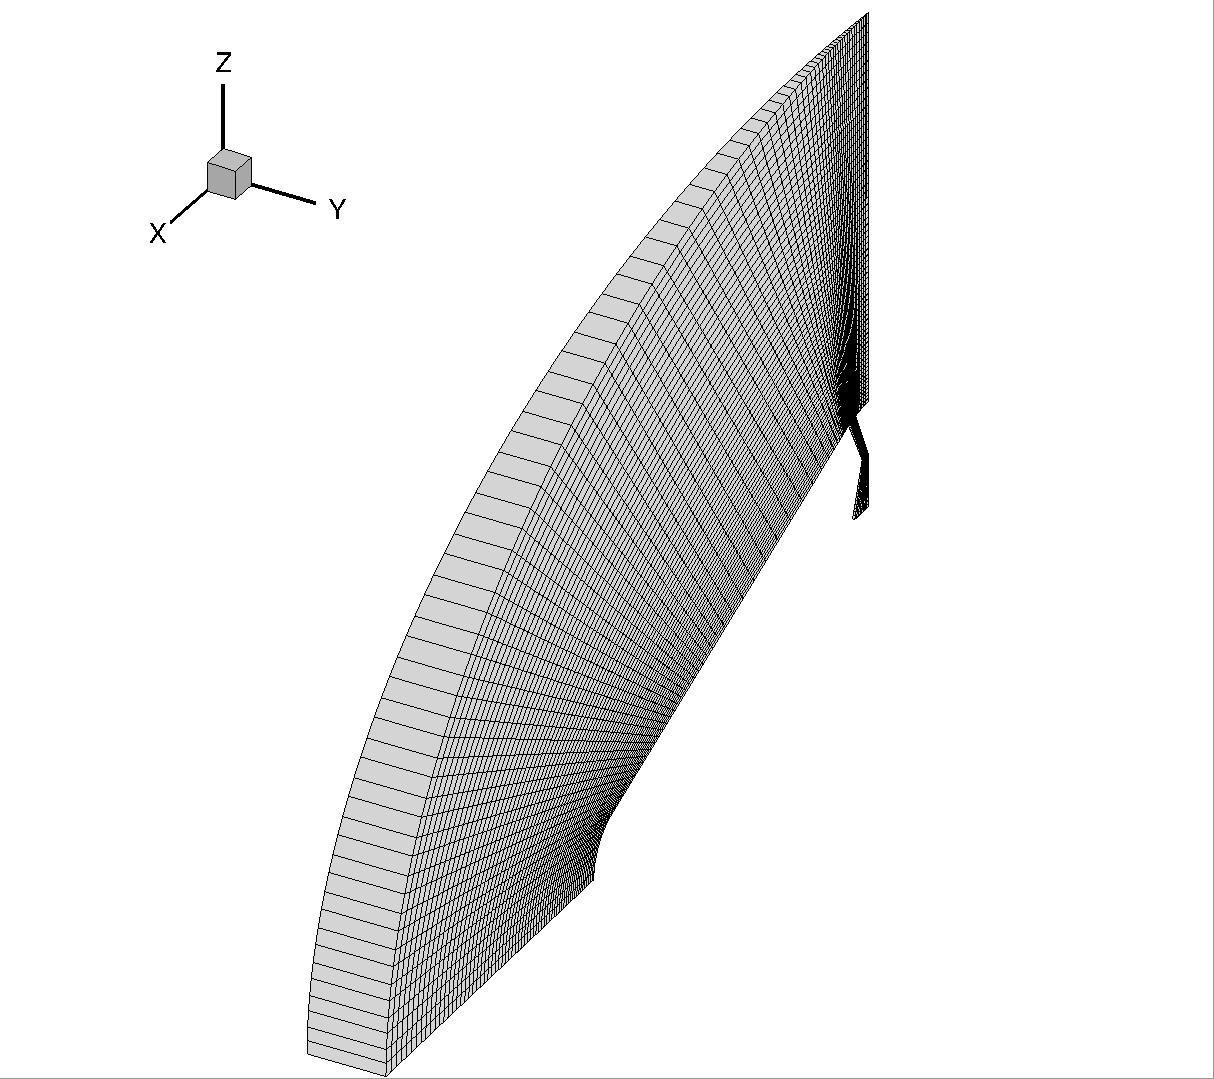
\includegraphics[width=\textwidth]{figures/all_iso.png}
  \end{subfigure}
	\begin{subfigure}[b]{0.4\textwidth}
    \centering
    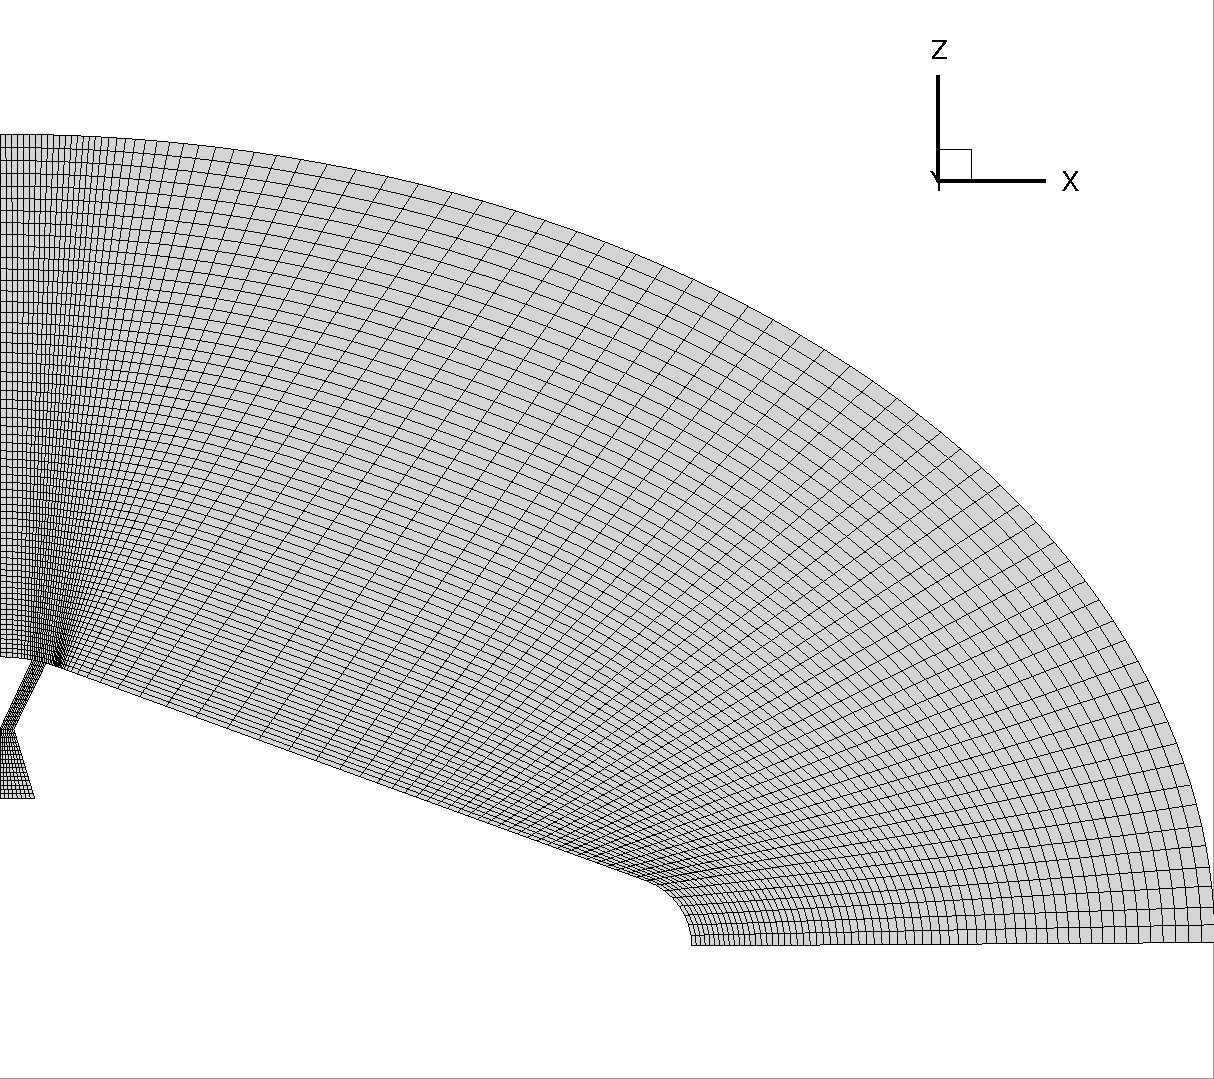
\includegraphics[width=\textwidth]{figures/all_side.png}
  \end{subfigure}
  \caption{Annular Jet Geometry}
  \label{fig:annular-jet-side}
\end{figure}
%------------------------------------------------------------------------------%
This geometry was originally investigated by Gnoffo et
al\cite{gnoffo2016tapping} to obtain increased drag from ``pulsing'' the annular
jet to obtain a beneficial effect from the unsteady shock interaction with the
plume of the jet.  For this work, the optimization is conducted for purely steady
flow, with the intent of altering the plenum conditions to achieve the optimum
condition of maximizing drag, while minimizing surface temperature.

The geometry was generated with the parameters shown in \tref{tab:annular-geom},
with the mesh originally created as structured grid and then converted to an
unstructured grid of hexahedral elements.
%------------------------------------------------------------------------------%
\begin{table}[h]
  \centering
  \begin{tabular}{c|c|c}
    Parameter & Description & Value \\
    \hline
    $r_{throat}$       &   nozzle throat radius, $m$           & 0.02 \\
    $r_{plenum}$       &   nozzle radius at plenum face, $m$   & 0.05 \\
    $r_{exit,inner}$   &   inside nozzle radius at exit, $m$   & 0.03 \\
    $r_{exit,outer}$   &   outside nozzle radius at exit, $m$  & 0.05 \\
    $l_{conv}$         &   distance from plenum to thoat, $m$  & 0.05 \\
    $\theta_c$         &   cone half angle, deg                & 70.0
  \end{tabular}
  \caption{Annular Nozzle Geometry Inputs}
  \label{tab:annular-geom}
\end{table}
%------------------------------------------------------------------------------%
The flow conditions for the optimization are shown in \tref{tab:flow-conditions}
%------------------------------------------------------------------------------%
\begin{table}[!h]
  \centering
  \begin{tabular}{c|c|c}
    Flow Condition & Description & Value \\
    \hline
    $V_{\infty}$    & freestream velocity, $m/s$        & 5686.24 \\
    $\rho_{\infty}$ & freestream density, $kg/m^3$      & 0.001 \\
    $T_{\infty}$    & freestream temperature, $K$       & 200.0 \\
    $M_{\infty}$    & freestream Mach number (derived)  & 20.0
  \end{tabular}
  \caption{Flow Conditions}
  \label{tab:flow-conditions}
\end{table}
%------------------------------------------------------------------------------%
\section{Cost Function Definition}

The cost function (or objective function) as formulated in FUN3D is a composite,
weighted function
%------------------------------------------------------------------------------%
\begin{equation}
  f = \sum_{j=1}^{N_{func}}w_j\left( C_j - C_{j^*} \right)^{p_j}
  \label{generic-cost-function}
\end{equation}
%------------------------------------------------------------------------------%
Where $w_j$, $C_{j^*}$, and $p_j$ are the weight, target, and power of cost
function component $j$.  $C_j$ is the component value, which is evaluated at
each flow solution.  For this particular optimization problem the cost function
is defined as 
%------------------------------------------------------------------------------%
\begin{equation}
  f = w_1\left( T_{RMS} \right)^{2} + w_2\left( C_{D} - C_{D}^{*} \right)^2
  \label{cd-tt-cost-function}
\end{equation}
%------------------------------------------------------------------------------%
The component weights were determined heuristically, to normalize the changes in
drag coefficient, $C_D$, and surface temperature Root-Mean-Square (RMS) $T_{RMS}$.
The drag coefficient is defined as
%------------------------------------------------------------------------------%
\begin{equation}
  C_D = \sum_{i}^{N_{faces}}
        \frac{2\left( p_i - p_\infty \right)n_{x_{i}}}
        {\rho_{\infty} V_{\infty}S_{ref}}
  \label{drag-coef-def}
\end{equation}
%------------------------------------------------------------------------------%
where $p_i$ is the average pressure at face $i$.  RMS of surface temperature is
defined as
%------------------------------------------------------------------------------%
\begin{equation}
  \sqrt{
    \frac{\sum_{i}^{N_{faces}}\left( T_{RMS} A_i \right)^2}
       {\sum_{i}^{N_{faces}}\left( A_i \right)^2}
     }
  \label{tt-rms-def}
\end{equation}
%------------------------------------------------------------------------------%
The area-weighted RMS of surface temperature was chosen over a simple
area-weighted average of surface temperature, because the stagnation temperature
is generally much higher than temperature elsewhere on a vehicle forebody in
hypersonic flows; therefore, the squaring of temperature in the RMS will give
greater weight to the stagnation temperature in the design.

%------------------------------------------------------------------------------%
\begin{figure}[h]
  \centering
	\begin{subfigure}[b]{0.4\textwidth}
    \centering
    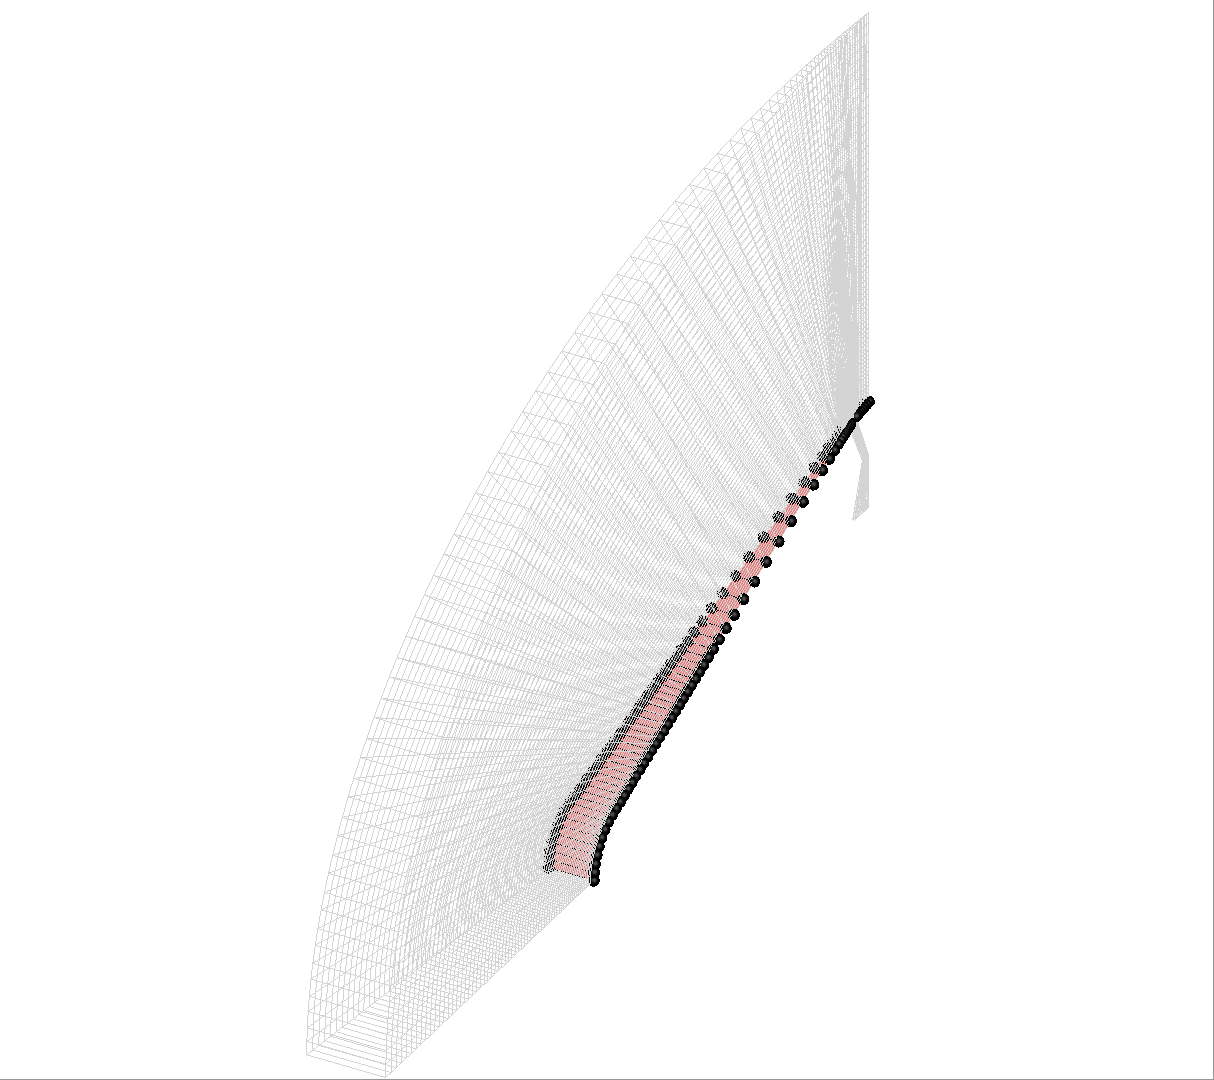
\includegraphics[width=\textwidth]{figures/surface2.png}
    \caption{$C_D$ and $T_{RMS}$ Integrated Area}
    \label{fig:cd-t-rms-area}
  \end{subfigure}
	\begin{subfigure}[b]{0.4\textwidth}
    \centering
    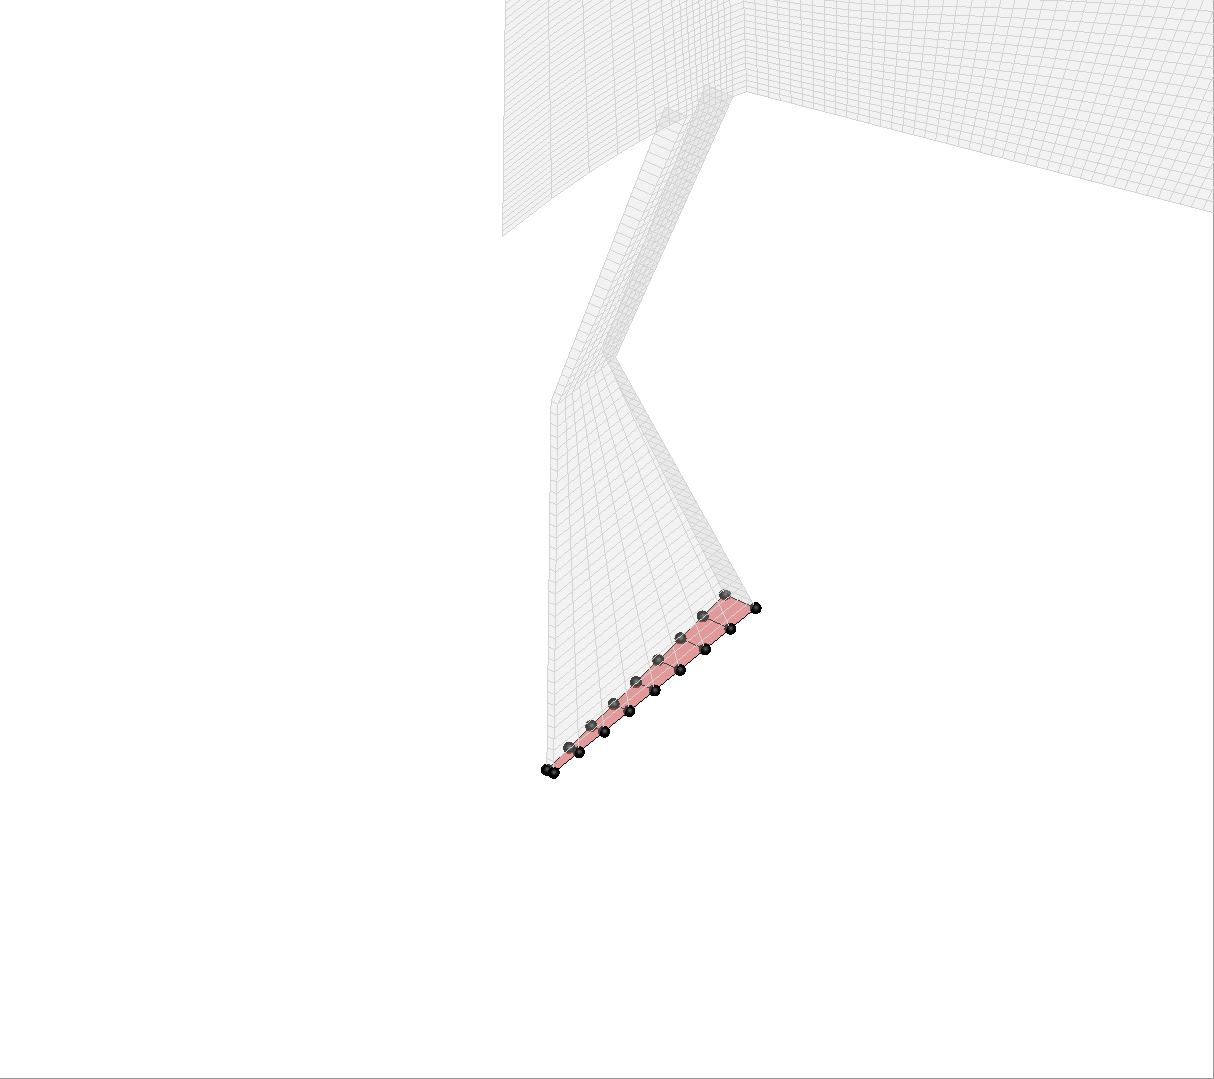
\includegraphics[width=\textwidth]{figures/plenum_bc.png}
    \caption{Plenum Face Boundary Condition}
    \label{fig:plenum-face}
  \end{subfigure}
\end{figure}
%------------------------------------------------------------------------------%

A primary objective of this optimization is to explore the effects of the plume
from the annular jet interacting with the bow shock; thus, the thrust effects
and, therefore, forces inside the nozzle are ignored.  To accomplish this, only
the area shown in \fref{fig:cd-t-rms-area} is integrated to compute the drag
coefficient and surface temperature RMS.


\section{Design Variables}

The design variables for the optimization problem are the plenum total pressure,
$P_{p,o}$, and plenum total temperature, $T_{p,o}$.  These are provided
explicitly in the optimization problem, and are used to directly set the flow
conditions on plenum face boundary condition in the nozzle, shown in
\fref{fig:plenum-face}.  For a reacting gas mixture, mass fractions for species
leaving the plenum can also be specified as a design variable.

The sensitivity gradients for these design variables are easily obtained by
manipulating \eref{obj-function} to obtain
%------------------------------------------------------------------------------%
\begin{equation}
  \pd{L}{\md} = \pd{f}{\md} + \rtdiff{}{\mq} \mathbf{\Lambda}
  \label{obj-linearization}
\end{equation}
%------------------------------------------------------------------------------%
Thus once the adjoint co-state variables $\mathbf{\Lambda}$ has been computed by
by solving the adjoint equations (\eref{adjoint-main}) the sensitivity
derivatives for $C_D$ and $T_{RMS}$ on the specied surfaces are obtained by
evaluating relatively inexpensive matrix-vector products.
